\section{Diode}
\subsection*{Durchführung}
Am Anfang dieses Versuchsteils bestimmten wir Sperr"~ und Durchlassrichtung der Diode. Dann nutzten wir das gegebene Programm um die Diodenkennlinie aufzunehmen.

\subsection{Grundlagen - Diodengleichung}

Die auch Shockley-Gleichung genannte Diodengleichung ist: 

\begin{eqnarray}
\label{eq:shockley}
I_\text{D} = I_\text{S}(T) \, \left(\mathrm e^\frac{U}{n\,U_\text{T}} - 1 \right)
\end{eqnarray}

$I_\text{S}(T)$ bezeichnet den Sättigungssperrstrom, $ U_\text{T}= \frac{k \cdot T} q$ die Tem\-pe\-ra\-tur\-span\-nung und $n$ den Idealitätsfaktor. Dieser soll bestimmt werden. 

In unserem Fall (Raumtemperatur) beträgt die Temperaturspannung  ${U_\text{T}=25}$\,mV.

\subsection*{Rechnung - Idealitätsfaktor}

Durch Variation der angelegten Spannung erhalten wir Abbildung \ref{fig:diode}. Dafür wurde die rechte Seite der Grafik mit der Shockley-Gleichung gefittet. Der Idealitätsfaktor kann dann über den Parameter B bestimmt werden:

\begin{figure}[t]
    \centering
    \includegraphics[width=\linewidth]{data/Diode.png}
    \caption{Diodenkennline}
    \label{fig:diode}
\end{figure}

\begin{eqnarray}
    n=\frac{e}{BkT}=\frac{e}{13.44\frac{J}{C}k\cdot300K}\approx2.88
\end{eqnarray}

\subsection*{Fehllerrechnung - Idealitätsfaktor}
Um den Fehler durch Fehlerfortpflanzung zu bestimmen nehmen wir den auf dem Fit gegebenen Wert für den angepassten Parameter $\frac{1}{nU_\text{T}}$, welchen origin uns mit $\Delta(n U_T)^{-1}=\pm 0.687$ angibt.
Der Gesammtfehler beträgt somit:
\begin{eqnarray}
    \Delta n = \left|\frac{\partial n}{\partial B)}\right|\Delta B= \left|\frac{e}{B^2kT}\right| \Delta B=\frac{e}{13.44^2\frac{J^2}{C^2}k\cdot300K}\cdot0.69\frac{J}{C}\approx0.15
\end{eqnarray}

\subsection*{Ergebnis - Idealitätsfaktor}
Der bestimmte Idealitätsfaktor der Diode ist somit:
\begin{eqnarray}
    n = (2.88\pm0.15)
\end{eqnarray}
Typische Idealitätsfaktoren für ideale Dioden liegen im Bereich 1-2. Wir haben also keine ideale Diode vorliegen.

\subsection*{Rechnung - Durchschlagsspannung}
Um die Durchschlagsspannung zu bestimmen fitten wir den lienaren Ansatz $I(U)=B\cdot U + A$ an den Bereich der starken Steigung auf der Sperrichtungsseite. Der Betrag des horizontalen Achsenabschnitts ist die gesuchte Spannung. 

Aus der Messung (siehe Grafik \ref{fig:diode}) ergeben sich die Werte $A=458.08$\,mA und $B=125,26\,\frac{1}{\Omega}$, die mit der Gleichung $I=B \cdot U_D + A \stackrel{!}{=} 0$ 
$$U_D = \frac{-A}{B}  \approx -3.66\,\mathrm{V}$$ ergeben.

\subsection*{Fehlerrechnung - Durchschlagsspannung}

Aus Origin werden folgende Fehler für B und A gegeben:$\Delta B = \pm 10.61$ und $\Delta A = \pm43.58$.

Erneut durch Fehlerfortpflanzung erlangen wir:
\begin{eqnarray}
    \Delta U =\left|\frac{\partial U_D}{\partial B}\right| \Delta B + \left|\frac{\partial U_D}{\partial A}\right|\Delta A = \left|\frac{A\Delta B}{B^2}\right|  + \left|\frac{\Delta A}{B}\right| \approx0.66 \mathrm{V}
\end{eqnarray}


\subsection*{Ergebnis - Durchschlagsspannung}
Die bestimmte Durchschlagsspannung ist:
\begin{eqnarray}
    U_D = (-3.66\pm 0.66)\mathrm{V}.
\end{eqnarray}
Dieser Wert lässt darauf schließen, dass es sich bei der untersuchten Diode um eine Zener-Diode handelt: Diese Dioden werden beim Betrieb in Sperrrichtung nicht zerstört und lassen sich beispielsweiese als Spanungsstabilisatoren einsetzen.

\section{Bipolartransistor}
\subsection*{Durchführung}

\textbf{Ab hier stehen uns fremde Messdaten zur Verfügung, da das Messgerät aufgab.}

\subsection{Grundlagen}
Um einen Bipolartransistor zu klassifizieren, werden die vier relevanteren Kombinationen der Größen $\text{I}_\text{E} , \text{I}_\text{C} , \text{I}_\text{B} , \text{U}_{\text{CE}} , \text{U}_{\text{BE}} \text{ und }\text{U}_\text{C} $ aufgetragen. Dies ist in Abbildung \ref{fig:bpt} geschehen.

Die Vierpolparameter als Ele\-mente der $U_{1,2}$ mit $I_{1,2}$ verbindenden Matrix definiert.
\begin{eqnarray}
    \begin{pmatrix}
        \text{U}_1\\
        \text{I}_2
    \end{pmatrix}=
    \begin{pmatrix}
        \text{h}_{11}&\text{h}_{12}\\
        \text{h}_{21}&\text{h}_{22}
    \end{pmatrix}\cdot
    \begin{pmatrix}
        \text{I}_1\\
        \text{U}_2
    \end{pmatrix}.
\end{eqnarray}

Hierbei ist:
\begin{description}
\item{h$_{11}$} die Kurzschluss-Eingangsimpedanz,
\item{h$_{12}$} die Leerlauf-Spannungsrückwirkung,
\item{h$_{21}$} die negative Kurzschluss-Stromübersetzung und 
\item{h$_{22}$} die Leerlauf-Ausgangsadmittanz.
\end{description}
Mit dem von uns gewählten Arbeitspunkt ($\text{U}_\text{CE} = 2$V und $\text{I}_\text{B}=0,2$mA) bestimmen wir die folgenden Werte durch Annäherung der einzelnen Sektoren durch lineare Funktionen:
\begin{align}
h_{11}=&\frac{\partial U_{BE}}{\partial I_B}=(77,3\pm5,3)\,\Omega\notag\\
h_{12}=&\frac{\partial U_{BE}}{\partial U_{CE}}=(-0,0038\pm0,0001)\notag\\
h_{21}=&\frac{\partial I_C}{\partial I_B}=(179,28\pm1,85)\notag\\
h_{22}=&\frac{\partial I_C}{\partial U_{CE}}=\frac{0,817\pm0,018}{k\Omega}\notag
\end{align}


Die angegeben Fehler sind die der Fitparameter.
\begin{figure}[t]
    \centering
    \includegraphics[width=\linewidth]{data/kennlinieBPT.png}
    \caption{Kennlinienfeld des Bipolartransistors}
    \label{fig:bpt}
\end{figure}


\section{Feldeffekttransistor}

Die in Abbildung \ref{fig:fet} dargestelten Kennlinien eines Metall-Oxid-Halbleiter-Feldeffekttransistor (FET) belegen, dass es ein selbstsperrender ist, da bei abnehmender Drain-Source-Spannung der Drain-Source-Strom abnimmt.

Auf der linken Seite der Grafik ist das Eingangsfeld, auf der rechten Seite das Ausgangsfeld dargestellt. Im Falle des Eingangsfeldes ist die Gate-Source-Spannung $U_{GS}$ gegen den Strom aufgetragen, beim Ausgangsfeld die Drain-Source Spannung $U_{DS}$.

\begin{figure}[t!]
    \centering
    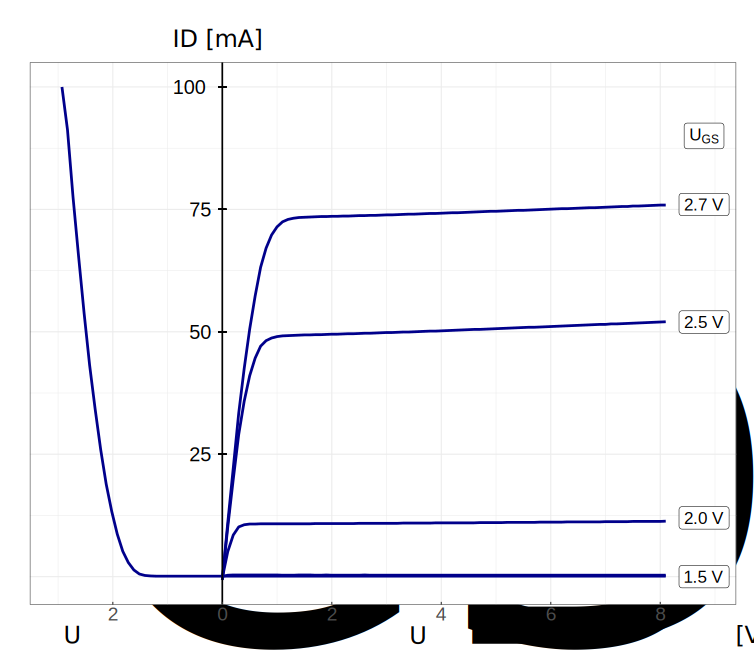
\includegraphics[width=\linewidth]{data/FET.png}
    \caption{Kennlinienfeld des Feldeffekttransistors}
    \label{fig:fet}
\end{figure}

\section{Solarzelle}

\subsection*{Grundlagen - wichtige Kenngrößen}
\begin{description}
\item[Das Strom-/Spannungsverhältnis] ist durch 
\begin{eqnarray}\label{eq:photo1}
    I(U)=I_S\left( e^{\frac{eU}{nkT}} -1 \right) - I_P
\end{eqnarray}
näherungsweise beschrieben. Die Gleichung entspricht bis auf $I_P$ (Photostrom) der Diodengleichung.
\item[Die Leerlaufspannung] ist als die ohne Stromfluss durch die Solarzelle erzeugte Potentialdifferenz definiert. $\rightarrow I(U_{OC})\stackrel{!}{=}0$ Wenn man dies in Gleichung \ref{eq:photo1} einsetzt ergibt sich:
$$U_{OC}=\frac{kT}{e}\ln\frac{I_P}{I_S}$$
\item[Der Kurzschlussstrom] ist der Strom, der ohne anliegende Spannung fließt.
$$I_{SC}=I(0)=I_S\left( e^{\frac{e\cdot0}{nkT}} -1 \right) - I_P=I_S\left(1-1 \right) - I_P=-I_P.$$
Der negierte Photostrom entspricht also dem Kurzschlusstrom
\item[Der Maximum-Power-Point] ist der Punkt der maximalen Leistung $P_{Max}$ einer Solarzelle. Um ihn zu erreichen gilt es $P=I\cdot U$ zu maximieren.
\item[Der Füllfaktor] $FF=\frac{P_{MPP}}{I_{SC}\cdot U_{OC}}$ ist ein Gütekriterium. Er sollte nahe 1 liegen.
\item[Der Wirkungsgrad] ist der Quotient aus maximaler Leistung und durch die Bestrahlung gegebenen:$$\eta=\frac{P_{MPP}}{P_{Ein}}$$
\end{description}

\subsection{Dunkelkennlinien}

Die Gleichung der Dunkelkennlinie ist äquivalent zur Diodengleichung \ref{eq:shockley}. Nach Rechnungen und Fits gleicher Art, wie zuvor im Versuchteil der Dioden erhalten wir folgende Ergebnisse:
\subsubsection{Monokristalline Solarzelle}

$$
    n=\frac{e}{BkT}=\frac{e}{17.84\frac{J}{C}\cdot k\cdot 300K}=2.17        
$$
$$
    \Delta n=\left|\frac{e}{B^2kT}\right| \Delta B=\frac{e}{17.84^2\frac{J^2}{C^2}k\cdot300K}\cdot0.14\frac{J}{C}\approx0.02
$$
$$
    \Rightarrow n=2.17\pm0.02
$$
\noindent Die Kennlinie ist in Abbildung \ref{fig:monokrisdunkel} zu sehen. Die Ähnlichkeit zur idealen Diode lässt sich auf den strukturellen Aufbau der Zelle zurückführen.\\

\begin{figure}[h!]
    \centering
    \includegraphics[width=\linewidth]{data/MonoDunkel.png}
    \caption{Dunkelkennlinie der monokristallinen Solarzelle}
    \label{fig:monokrisdunkel}
\end{figure}

\subsubsection{Amorphe Solarzelle}

$$
    n=\frac{e}{BkT}=\frac{e}{0.69\frac{J}{C}\cdot k\cdot 300K}=56.06        
$$
$$
    \Delta n=\left|\frac{e}{B^2kT}\right| \Delta B=\frac{e}{0.69^2\frac{J^2}{C^2}k\cdot300K}\cdot0.002\frac{J}{C}\approx0.16
$$
$$
    \Rightarrow n=56.06\pm0.16
$$

\noindent Die Kennlinie ist in Abbildung \ref{fig:amodunkel} zu sehen. Die amorphe Solarzelle zeigt starke Abweichungen zur idealen Diode auf. Dies ist auch zu erwarten, da in der Zelle keine Fernordnung existiert, und sie somit einer idealen Diode recht unähnlich ist.\\

\begin{figure}[h]
    \centering
    \includegraphics[width=\linewidth]{data/AmorphDunkel.png}
    \caption{Dunkelkennlinie der amorphen Solarzelle.}
    \label{fig:amodunkel}
\end{figure}


\subsection{Hellkennlinien}

Aus dem Graph der Hellkennlinie, lassen sich die anderen Werte ablesen:

\begin{description}
\item[Der Kurzschlussstrom] I$_{SC}$ ist der Achsenabschnitt der vertikalen Achse, der nach Ablesen noch durch die Fläche der Zelle zu teilen ist. Im Fall der amorphen Zelle ist für diesen und andere Werte entweder ein Faktor (Strom) oder Divisor (Spannung) 5 hinzuzufügen, da es sich um fünf Einzelzellen handelt.
\item[Die Leerlaufspannung] U$_{OC}$ ist der Achsnabschnitt der horizontalen Achse.
\item[Der Füllfaktor] ergibt sich aus dem Minimum der Leistungs-Spannungs-Kurve. Der Punkt dieser Stelle im I-U-Diagramm ist der MPP. Der Füllfaktor ist dann $Ff=\frac{I_{MP}U_{MP}}{I_{SC}U_{OC}}$.
\item[Der Wirkungsgrad] ist $\mu=\frac{\text{maximale Leistung}}{\text{Lichtleistung}}$.
\end{description}


\subsubsection{Monokristalline Solarzelle}

\paragraph{Leerlaufspannung}
$$
    U_{OC} =& 0,4955\,\text{V}
$$

\paragraph{Kurzschlussstrom}
$$|\frac{I_{SC}}{A}|=\frac{28,995\,\text{mV}}{25\Text{cm}^2}=1,160\,\frac{\text{mA}}{\text{cm}^2}$$

\paragraph{MPP} Siehe hierzu Graph \ref{fig:sol-mon-p}
$$U_{MP}=0,39\,\text{V}$$ $$\vert I_{MP}\vert=24,658\,\text{mA}$$ 
Dieser Punkt impliziert eine Leistung von 9,37mV.

\paragraph{Füllfaktor}

$$    Ff=\frac{I_{MP}U_{MP}}{I_{SC}U_{OC}}=\frac{99,1\,\text{mV}\cdot144,775\,\text{mA}}{390\,\text{mV}\cdot24,658\,\text{mA}}=65,3\%   $$

\paragraph{Der Wirkungsgrad} ist über die Leistung der Lampe zu errechnen. Diese strahlt in Summe 150W aus. Die Solarzelle ist 44,7cm von der Lampe entfernt und mit einem Flächeninhalt von 25cm$^2$ ergibt sich so eine Lichtleistung von $150W\cdot\frac{25cm^2}{12554cm^2}=0,300W$

Der Wirkungsgrad ist somit:
$$
\eta=\frac{I_{MP}U_{MP}}{P_{Ges}A}=\frac{9,37\,\text{mW}}{300\,\text{mW}}=3,12\%.
$$
Die Kennlinie ist in Abbildung \ref{fig:monokrishell} zu sehen.\\

\begin{figure}[t!]
    \centering
    \includegraphics[width=\linewidth]{data/MonoLicht}
    \caption{Hellkennlinie der monokristallinen Solarzelle.}
    \label{fig:monokrishell}
\end{figure}


\subsubsection{Amorphe Solarzelle}
Wir gehen hier davon aus, dass die Fläche von 6cm$^2$ auf alle fünf Zellen bezogen ist.
\paragraph{Leerlaufspannung}
$$
    U_{OC} =\frac{3,15\,\text{V}}{5}=630\,\text{mV}
$$

\paragraph{Kurzschlussstrom}
$$ \frac{I_{SC}}{A}=\frac{5\cdot0,781\,\text{mA}}{\frac{6}{5}\,\text{cm}^2} =3,254\,\frac{\text{mA}}{\text{cm}^2 }$$

\paragraph{MPP} Siehe hierzu Graph \ref{fig:sol-amo-p}
$$
    U_{MP}=\frac{2,1}{5}\,\text{V}=0,42\,\text{V}\\
    \vert I_{MP}\vert=3,49\,\text{mA}
$$
mit einer Leistung von 1,4643mV

\paragraph{F"ullfaktor}

$$    Ff=\frac{I_{MP}U_{MP}}{I_{SC}U_{OC}}=\frac{0,99\,\Text{mW}}{5\cdot0,781\cdot\frac{3,15}{5}\,\text{mW}}=40,2\%$$

\paragraph{Der Wirkungsgrad} ist erneut über die Leistung der Lampe zu errechnen. Diese strahlt 150W aus. Die Solarzelle ist 41,7cm entfernt und mit einem Flächeninhalt von in Summe 6cm$^2$ ergibt sich so eine Lichtleistung auf allen fünf Solarzellen von $150W\cdot\frac{6cm^2}{262,01cm^2}=3,43\,\text{W}§

Der Wirkungsgrad ist somit:
$$
\eta=\frac{I_{MP}U_{MP}}{P_{Ges}A}=\frac{1,4364\,\text{mW}}{\frac{3,43}{5}\,\text{W}}=0,2\%.
$$
Die Kennlinie ist in Abbildung \ref{fig:amorphkrishell} zu sehen.\\

\begin{figure}[t!]
    \centering
    \includegraphics[width=\linewidth]{data/AmorphLicht.png}\caption{Hellkennlinie der amorphen Solarzelle.}
    \label{fig:amorphkrishell}
\end{figure}